\section{Noción de identidad.} \label{identity}

La matriz identidad $I$ es aquélla que cumple que $AI = IA = A$. Es interesante buscar una noción similar en las cubrices, sin embargo, pronto descubrimos que nuestras expectativas sobre esta se ven desafiadas.

\subsection{Unicidad de I.} \label{identity-unique}

Sean $A, I \in M_{n} (\mathbb{K})$ tal que $IIA = A$ (el razonamiento funciona independientemente del orden del producto). Partimos de tres asunciones:

\begin{itemize}
	\item Ningún elemento de $A$ es nulo.
	\item Los elementos de $I$ no dependen de los de $A$.
	\item La cubriz identidad $I$ es única.
\end{itemize}

Por definición:

$$A_{ijk} = (I \cdot I \cdot A)_{ijk} = \sum\limits_{l=1}^{n} I_{ilk} \cdot I_{ljk} \cdot A_{ijl}$$

Como suponemos que $I$ no depende de $A$, la expresión solo puede producir $A_{ijk}$ a partir del término $A_{ijl}$ del sumatorio. En otras palabras, $I_{ilk} I_{ljk} = \delta_{lk}$, donde $\delta_{lk}$ es la \textit{delta de Kronecker}, una expresión que utilizaremos frecuentemente y que equivale a:

\begin{equation}
	\delta_{ab} =
	\begin{cases}
		1 & \text{si } a = b \\
		0 & \text{si } a \neq b
	\end{cases}
\end{equation}

En base a las anteriores expresiones podemos derivar una fórmula para $I_{ijk}$ manipulando sutilmente los subíndices. Véase $I_{ilk}$ y nótese que decir que es igual a $1$ si $l$ toma el valor de $k$ es equivalente a decir que es igual a $1$ si su $j$ es igual a su $k$. En otras palabras, $I_{ijk} = \delta_{jk}$. Pero aplicando el mismo razonamiento sobre $I_{ljk}$ obtenemos que $I_{ijk} = \delta_{ik}$. La única manera de evitar esta contradicción es establecer que $I_{ijk} = \delta_{jk} \delta_{ik}$, pero esto necesariamente excluye múltiples elementos de $A$. (Véase el Apéndice \ref{appendix-1} para un desarrollo completo en el caso particular $M_2 (\mathbb{K})$ si se precisa esclarecer el patrón).

Al menos una de nuestras suposiciones debe estar errada, y sería óptimo que fuese la tercera (sobre la unicidad de la identidad).

\subsection{La identidad como par.} \label{identity-pair}

Decimos que $I, J \in M_{n} (\mathbb{K})$ forman un \textit{par identidad} si cumplen que $AIJ = A$ (exploraremos más adelante la influencia del orden de los factores). Nuevamente utilizamos la definición del producto:

$$A_{ijk} = (AIJ)_{ijk} = \sum\limits_{l=1}^{n} A_{ilk} I_{ljk} J_{ijl}$$

Esta vez las condiciones a satisfacer son:

\begin{itemize}
	\item $I_{ljk} = J_{ijl}^{-1}$ para $l = j$ y $I_{ljk} J_{ijl} = 0$ para $l \neq j$.
	\item $J_{ijl} = I_{ljk}^{-1}$ para $l = k$ y $J_{ijl} I_{ljk} = 0$ para $l \neq k$.
\end{itemize}

Dos cubrices cualquiera que cumplan estas condiciones serán consideradas un \textit{par identidad}, y cumplirán que $AIJ = A$. Es evidente entonces que si $\mathbb{K}$ es un cuerpo, existirán infinitos pares identidad, mientras que si es un anillo unitario conmutativo, solo existirán los que a continuación presentamos.

\subsection{Las tres Kronecker.} \label{identity-kronecker}

Por comodidad y estandarización, resulta inmediata la idea de establecer que todos los términos que deban ser el inverso de otros términos sean iguales a $1$, mientras que todos los que deban anularse con otro sean iguales a $0$.

Es decir, que para que $(AIJ)_{ijk} = A_{ijk}$, debe cumplirse que $I_{ljk} = J_{ijl} = \delta_{jl}$. Con un razonamiento muy similar al de la sección \ref{identity-unique}, podemos independizar estas expresiones del subíndice $l$:

$$I_{ijk} = \delta_{ij}$$

Teniendo en cuenta que el par identidad no es conmutativo, es sencillo hacer un desarrollo similar tanto para $I_2 A J_2$ como para $I_3 J_3 A$ (conmutar la posición de $I$ y $J$ no produce nuevas cubrices, solo conmuta sus nombres). Tomando $\Delta_{ab} = (\delta_{ab})$, obtenemos que: %, de lo cual obtendremos que:

$$A = A \Delta_{ij} \Delta_{jk} = \Delta_{ij} A \Delta_{ik} = \Delta_{jk} \Delta_{ik} A$$

Con esto concluímos que existen tres pares identidad estándar fundamentados sobre las tres Kronecker. No es inmediatamente obvio qué patrón se puede esclarecer de este resultado. Sea como fuere, es intrigante observar las cubrices dibujadas por cada Kronecker. Tomemos sus representaciones tridimensionales completas.

\begin{figure}[H]
	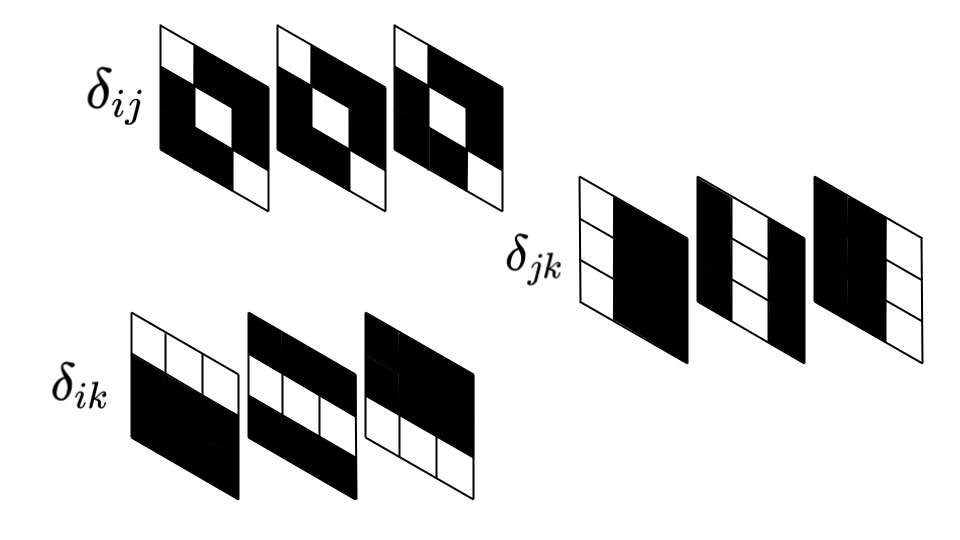
\includegraphics[width=\linewidth]{media/kroneckers.png}
	\caption{Representación tridimensional completa de $\Delta_{ij}$, $\Delta{jk}$ y $\Delta{ik}$ (celdas iguales a $1$ en blanco e iguales a $0$ en negro).}
\end{figure}

Puede ser útil reagrupar y renombrar los términos de la siguiente forma. Si $I_{ijk} = 1$, entonces:

\begin{itemize}
	\item $A = A \Delta_{ij} I = A I \Delta_{jk}$.
	\item $A = \Delta_{ij} A I = I A \Delta_{ik}$.
	\item $A = \Delta_{jk} I A = I \Delta_{ik} A$.
\end{itemize}
